%% ----------------------------------
%%   Kap03---Konzept.tex
%% ----------------------------------

%% eigenes Konzept, Lösungsansatz für das Erreichen der Zielsetzung aus Kap. 1

\chapter{Konzept}
\label{sec:Chapter3}

In diesem Kapitel wird auf das Konzept dieser Arbeit eingegangen. Es wird in den folgenden Abschnitten darüber gesprochen, welches Qualitätsmaß für die Memristoren gewählt wurde und nach welchem Konzept dieses Qualitätsmaß in der Folge implementiert werden soll. Außerdem wird in den folgenden Abschnitten erklärt, warum solch ein Qualitätsmaß gewählt wurde und wieso andere Merkmale eines Memristors gar nicht oder nur sehr wenig betrachtet werden. Die Aufstellung des Qualitätsmaßes beginnt hierbei mit der Formbarkeit, gefolgt von dem Energieverbrauch. Danach folgt die Speichergröße als Qualitätsparameter. Als viertes wird die Lebensdauer eines Memristors approximiert. Dabei wird nochmal näher auf die Arbeit von Pouyan, Amat und Rubio~\cite{stat_lifetime} eingegangen. Neben dem Qualitätsmaß soll in diesem Kapitel auf die Ähnlichkeiten zwischen zwei Memristoren eingegangen werden. Dabei wird erklärt, worauf geachtet werden muss, auf welche Merkmale es dabei ankommt und wie dies in dieser Arbeit aufgenommen wird. Zuletzt wird noch der Einfluss des Materials auf die Qualität thematisiert.

\section{Bestimmung einer Qualitätsklasse für Memristoren}
  In diesem Abschnitt wird ein Qualitätsmaß für Memristoren definiert. Hierbei ist es erst einmal wichtig festzustellen, was die Qualität eines Memristors ausmacht. Doch wie genau ist Qualität überhaupt definiert? David A. Garvin hat bereits 1984 in seiner Arbeit~\cite{garvin_qual} festgestellt, dass es sehr viele verschiedene Definitionen von Qualität gibt, weshalb er diese in unterschiedliche Kategorien einteilte und somit erklärte, warum sich viele Experten nicht auf eine Definition einigen konnten. So kam er dabei zur Einsicht, dass die Vorstellung von Qualität immer von der betrachtenden Partei abhängt und somit immer verschiedene Fassetten aufweist. Da diese Einsicht jedoch nicht zum allgemeinen Verständnis eines übergreifenden Qualitätsbegriffes beiträgt, gibt es Institutionen, welche Normen und Qualitätsmaße vorgeben, an welche sich die Industrie halten kann, um \glqq qualitativ hochwertige\grqq\,Waren zu produzieren. Bei Soft- und Hardware handelt es sich meistens um die Normen ISO oder DIN.

  Im Fall von Memristoren lassen sich natürlich nicht direkt Qualitätskriterien des ISO oder DIN anwenden, da noch keine offiziellen Normen für Memristoren existieren. Dementsprechend werden in dieser Arbeit typische Qualitätsmerkmale auf Memristoren zugeschnitten. Dabei wird speziell darauf eingegangen was ein typischer Nutzer eines memristiven Systems benötigt. Die Wahl fällt somit auf den sogenannten \glqq User-based Approach\grqq, um die Qualität zu definieren. Was erwartet der Nutzer eines Memristors also von seinem System? Bei einem Memristor handelt es sich um ein Speichermedium. Dementsprechend erwartet der Nutzer einen möglichst großen Speicher. Für die meisten Nutzer ist auch ein niedriger Energieverbrauch ein wichtiges Kriterium, wenn es um die Qualität von Hardware geht. Die letzten beiden noch zu betrachtenden Qualitätsmerkmale sind die Lebensdauer und Formbarkeit, welche in den vorangegangen Kapiteln schon näher erläutert wurden, da sie eine besondere Rolle in dieser Arbeit spielen. Die Temperatur ist für viele Hardwarekomponenten ein weiteres Qualitätsmerkmal. In dieser Arbeit wird dieses Merkmal für Memristoren jedoch ignoriert, da Memristoren allgemein als sehr hitzebeständig gelten~\cite{vde_memristor}, weshalb der Einfluss der Temperatur auf die Qualität nicht betrachtet wird.

  Die Benotung der Qualität in dieser Arbeit soll auf eine für die meisten sehr intuitive Weise ablaufen. Während Knowm Inc. Memristoren nur in \glqq funktionsfähig\grqq\,und \glqq nicht funktionsfähig\grqq\,einteilt, wird in dieser Arbeit eine genauere Bewertung vorgenommen. Somit werden für einen Memristor Qualitätsstufen nach einem schulnotenähnlichem Prinzip gewählt:
  \begin{itemize}
    \item[] 1 - sehr gute Qualität
    \item[] 2 - gute Qualität
    \item[] 3 - befriedigende Qualität
    \item[] 4 - schlechte Qualität
    \item[] 5 - sehr schlechte Qualität
    \item[] 6 - nicht funktionsfähiger Memristor
  \end{itemize}
  Eine detaillierte Beschreibung, welche Eigenschaften ein Memristor erfüllen muss, um eine bestimmte Note zu erhalten, findet sich in den folgenden Abschnitten und in dem Kapitel~\ref{sec:Chapter4}. Dafür wird in den folgenden Abschnitten jede Teilnote, welche zu der Gesamtnote zwischen 1 und 6 führen, näher aufgeschlüsselt.

\subsection{Qualitätskriterium: Speichergröße}
\label{sec:Quali_Speicher}
  Dieser Abschnitt soll sich mit der Bestimmung und Kategorisierung der Speichergröße von Memristoren befassen. Wie ist also Speichergröße bei Memristoren festgelegt und wie genau kann diese Größe in Qualitätsmerkmalen festgehalten werden. Wie im Kapitel~\ref{sec:Chapter2} bereits beschrieben wurde, besitzen Memristoren die Eigenschaft, beim Anlegen einer bestimmten Spannung in einen höher- bzw. niedrigerresistenten Zustand zu wechseln, weil sich dabei Ionenkanäle bilden. Wenn keine Spannung an den Memristor angelegt wird, bleibt dieser in dem zuletzt erreichten Zustand, was ihm seine memristive Eigenschaft verleiht. Im Kapitel~\ref{sec:Chapter2} wird beschrieben, dass auf Memristoren basierende Systeme viel mehr Speicherplatz auf eine kleinere Chipfläche bringen können als herkömmliche Speichermedien. Doch welchen Einfluss hat das auf die Qualität?

  Kann man durch das Setzen eines Memristors beispielsweise 16 verschiedene Zustände erreichen, so kann man davon sprechen, dass der Memristor vier Bit speichern kann ($0000$ bis $1111$ = $0$ bis $15$). Möchte man mit solchen Memristoren zum Beispiel 64 Bit an Information speichern, so würde man 16 der gerade beschriebenen Memristoren benötigen. Im Falle von herkömmlichen 1-Bit DRAM Speicherzellen würde man 64 Bausteine für diese Menge an zu speichernden Information benötigen. Kann ein anderer Memristor nur 15 oder weniger Zustände erreichen, so ist dies nicht der Fall. Es werden also mehr Memristoren benötigt, um 64 Bit Informationen zu speichern. Dementsprechend sollten Memristoren eine bestimmte Menge von Zuständen erreichen können, um als qualitativ hochwertig zu gelten. Ein Memristor, welcher beispielsweise nur zwei Zustände erreichen kann, verliert also einen wichtigen Vorteil gegenüber einer klassischen DRAM Kondensator/Transistor Speicherzelle, welche auch ein Bit an Information speichern kann. Ein solcher Memristor wäre also offensichtlich von schlechter Qualität, da er nur noch den Vorteil der Persistenz gegenüber den herkömmlichen Speichermedien besitzt und den wichtigen Vorteil der Speicherkapazität pro Fäche verliert.

  Es liegt also nahe, die Qualität der Speichergröße von Memristoren klassisch in Bit-Größen einzuteilen. Ein Memristor, welcher eine unäre Speichergröße hat, also nur einen Zustand erreichen kann und somit kein Bit Speicherkapazität besitzt, wird als nicht funktionsfähig definiert. Ist der Memristor nur in der Lage zwei Zustände zu erreichen, so ist die Qualität in diesem Qualitätsmaß von einer sehr schlechte Qualität. Solange ein Memristor nicht in der Lage ist mindestens drei Bit zu codieren, er also nur drei oder vier Zustände erreichen kann ($00$, $01$, $10$, $11$), ist die Qualität immer noch eher schlecht. Eine befriedigende Qualität hat ein Memristor erst wenn er drei Bit codieren kann. Ein Memristor, der in der Lage ist 3.5 Bit zu codieren, also 9-15 Zustände erreichbar sind, hat bereits eine gute Qualität. Mit vier Bit Speichergröße hat der Memristor eine außergewöhnlich gute Qualität, da er ab dieser Zustandsmenge in der Lage ist ein Nibble zu speichern. Dies hat in der Praxis großen Wert, da mit zwei solcher Memristoren ein Byte gespeichert werden kann. Die Bewertung nach der Speichergröße wird in der Tabelle~\ref{tab:Speicher} dargestellt.
  \begin{figure}
    \centering
    \begin{tabular}{l|c|c|c|c|c|c}
      \textbf{Zustände} & $\geq16$ & $9-15$ & $5-8$ & $3-4$ & $2$ & $1$ \\\hline
      \textbf{in Bit} & $4$ & $3.5$ & $3$ & $2$ & $1$ & $0$ \\\hline
      \textbf{Note} & $1$ & $2$ & $3$ & $4$ & $5$ & $6$
    \end{tabular}
    \caption{Allgemeines Qualitätsmaß im Hinblick auf die Speichergröße eines Memristors.}
    \label{tab:Speicher}
  \end{figure}

  Aber wie kann die Menge an Zuständen eines Memristors bestimmt werden? Jeder Memristor besitzt einen sogenannten \glqq Threshold\grqq, Englisch für den \glqq Schwellenwert\grqq. Dieser Threshold stellt die benötigte Spannung, um in einen höher-/niedrigerresistenten Zustand zu wechseln, dar. Der Threshold muss zunächst bestimmt werden, um im Weiteren die Anzahl an Zuständen bestimmen zu können. Die genaue Herangehensweise zur Bestimmung des Thresholds wird in der Implementierung im Kapitel~\ref{sec:Chapter4} beschrieben. Steht der Threshold fest, so ist nun bekannt mit welcher Spannung ein sogenannter \glqq Puls\grqq\,auf den entsprechenden Memristor geschickt werden muss. Mit dieser Spannung bilden sich die Ionenkanäle, welche die Leitfähigkeit des Memristors verändern. Sei der zuvor bestimmte Threshold $t$, die Spannung, welche im Puls angelegt wird $s$ und sei $V_{max}$ die maximale Spannung, welche laut Knowm Datenblatt~\cite{knowm_comp_2019}~auf dem Memristor angelegt werden darf. So muss für $s$ und $t$ Folgendes gelten:
  \begin{align}
    t \leq s < V_{max} \label{eq_ts}
  \end{align}
  Die Formel~\ref{eq_ts} beschreibt also, in welchem Wertebereich die für den Puls gewählte Spannung liegen darf. Die Spannung muss höher sein, als der festgelegte Threshold, damit sich die Leitfähigkeit des Memristors durch den Puls verändert. Jedoch darf die Spannung nicht höher liegen, als der von Knowm festgelegte Wert, da sonst die Gefahr besteht, dass der Memristor durchgbrennt.

  Um im Weiteren die Anzahl der Zustände des Memristors bestimmen zu können, muss der Memristor zunächst in den Zustand mit dem höchsten Widerstand gebracht werden. Ist der Memristor in diesem Zustand kann nun mit Pulsen mit der zuvor festgelegten Spannung $s$ jeweils der Zustand mit dem nächst niedrigeren Widerstand erreicht werden. Der Vorgang kann in der Theorie auch in die andere Richtung durchgeführt werden. Der Memristor kann also auch zuerst in den Zustand mit dem niedrigsten Widerstand gebracht werden und danach mit Pulsen über der Spannung $s$ in den Zustand des nächsthöchsten Widerstandes gebracht werden. In dieser Arbeit wurde jedoch der erste Ansatz gewählt, da er weniger anfällig ist, den Memristor im Kategorisierungsprozess zu beschädigen. In hochohmigen Widerstandsbereichen kann der Memristor nur \glqq umgedreht\grqq\,werden. Dabei wechselt der Memristor die Richtung, in welche Spannung angelegt werden muss, um den Widerstand zu erhöhen oder zu verringern. Der Memristor selbst kommt jedoch nicht zu Schaden. In niedrigerohmigen Widerstandsbereichen kann es beim wiederholten Anlegen von Pulsen dazu kommen, dass der Widerstand des Memristors so niedrig wird, dass der Memristor durchbrennt und er in dem Zuge kaputt geht. Deshalb wird in dieser Arbeit der Memristor erst in einen maximal hohen Widerstandsbereich gebracht, um danach vorsichtiger in einen niedrigeren Widerstandsbereich zu pulsen. Zu Beginn wird davon ausgegangen, dass eine Spannung $s = t$ ausreicht, um den nächsten Zustand zu erreichen. Jedoch müssen davor noch Tests durchgeführt werden. Dabei muss getestet werden, ob sich der Threshold zum Wechseln des Zustandes über den Verlauf der verschiedenen Widerstandsbereiche eines Memristors verändern kann oder nicht. Ist dies der Fall, so müsste entweder $s$ leicht angehoben werden oder zunächst der höchste Threshold bestimmt werden.

  \begin{figure}
    \centering
      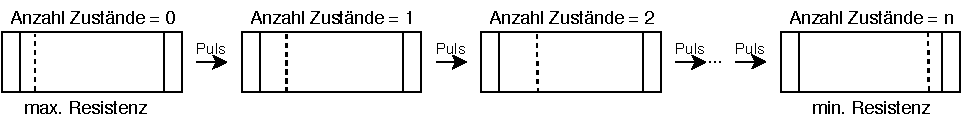
\includegraphics[width=0.95\textwidth]{images/Speicherbestimmung.pdf}
    \caption{Versinnbildlichung des Ablaufs zur Bestimmung der Anzahl der Zustände eines Memristors, wobei $n$ die mit der Methode bestimmte Anzahl an Zuständen darstellt.}
    \label{tab:Speicher_Noten}
  \end{figure}

  Für jeden Zustand, welchen man durch das Schalten eines Pulses erreicht, wird die Anzahl der Zustände erhöht. Dies wird solange durchgeführt, bis der Memristor den Zustand mit dem minimalen Widerstand erreicht. Hierbei muss jedoch darauf geachtet werden, dass der Memristor nicht durchbrennt, weil er unter den minimalen Widerstandsbereich gezwungen wurde. Wurde dieser Vorgang einmal durchlaufen, so hat man die Menge an Zuständen eines Memristors erhalten und kann diese Anzahl in das bereits beschriebene Bewertungskriterium einfügen. Der soeben beschriebene Ablauf kann natürlich auch mit den bereits genannten Risiken anders herum durchgeführt werden. Zuerst wird in diesem Fall der Zustand mit dem minimalen Widerstand gesucht und danach werden Pulse verwendet, um die Anzahl der Zustände bis zum Zustand mit dem maximalen Widerstand zu zählen.

\subsection{Qualitätskriterium: Energieverbrauch}
  Dieser Abschnitt befasst sich mit dem Energieverbrauch eines Memristors als Qualitätskriterium. Der Memristor gilt als energieeffizienter als herkömmliche Speichermedien~\cite{nonvolatile}.
  Jedoch braucht natürlich auch ein Memristor Strom, um zu funktionieren und somit muss der Energieverbrauch als Qualitätskriterium betrachtet werden. Dabei muss angemerkt werden, dass selbst ein Memristor mit relativ hohem Energieverbrauch im Vergleich zu den meisten herkömmlichen Speichermedien noch sehr energieeffizient ist.

  Doch wie misst man den Energieverbrauch eines Memristors und weist diesem einer Qualitätsklasse zu? Eine Möglichkeit wäre es, ein herkömmliches Amperemeter wie etwa einen Multimeter am Digilent Discovery Board anzuschließen. Damit kann der Strom gemessen werden, welcher fließt, wenn der Memristor benutzt wird. Der Energieverbrauch kann dann anhand der gemessenen Werte zusammen mit der angelegten Spannung berechnet werden und mit einer Norm für den Energieverbrauch von Memristoren abgeglichen werden und somit einer Qualitätsklasse zugeordnet werden.

  Zum aktuellen Zeitpunkt ist weder eine solche Norm bekannt, noch wurde eine wissenschaftliche Arbeit gefunden, in welcher der Energieverbrauch von einzelnen Memristoren festgehalten wurde. Somit wäre es von Nöten, eine solche Norm eigenständig aufzustellen. Eine solche Norm könnte wie folgt aufgestellt werden. Es müsste von jedem funktionsfähigem Memristor, welcher für diese Arbeit zur Verfügung gestellt wurde, der Strom gemessen werden. Aus den gemessenen Werten kann dann ein Mittelwert berechnet werden. Anhand dieses Mittelwertes kann wiederum ein Qualitätsmaß aufgestellt werden.

  Es gibt jedoch noch eine einfache Methode, um den Energieverbrauch eines Memristors zu bestimmen. Dafür muss zunächst erst einmal eine allgemeine Erklärung zur Bestimmung des Energieverbrauchs gemacht werden. Der Energieverbrauch wird in Watt gemessen. Die Berechnung dieser Leistung $P$ in Watt funktioniert unter der Anwendung der ohmschen Gesetze nach drei Formeln, wobei $I$ der Strom in Ampere, $R$ der Widerstand in Ohm und $U$ die Spannung in Volt darstellt. Die drei Formeln sehen wie folgt aus:
  \begin{align}
    P &= U \cdot I \label{align_p1}\\
    P &= I^2 \cdot R \label{align_p2}\\
    P &= \frac{U^2}{R} \label{align_p3}
  \end{align}
  Die Form zur Berechnung der Leistung aus Formel~\ref{align_p3} bietet sich für Memristoren am Besten an. Woran das liegt, soll im folgenden Absatz geklärt werden.

  Da Memristoren widerstandbasierende Bausteine sind, ist es logisch die Formel zu wählen, in welcher der Widerstand des Memristors als Faktor zur Berechnung der Leistung verwendet wird. Es gilt also zu klären, wieso sich die Form aus Formel~\ref{align_p3} besser eignet als die Formel~\ref{align_p2}. Dafür müssen einmal alle möglichen Operationen für Memristoren dargestellt werden. Ein Benutzer eines Memristors kann auf diesem effektiv zwei Operationen ausführen: Das \glqq Auslesen\grqq\,und das \glqq Setzen\grqq\,von Memristoren. Für beide Operationen wird eine gewisse Spannung auf dem Memristor angelegt. Beim Auslesen des Memristors wird eine sehr niedrig gewählte Spannung auf dem Memristor angelegt, um den Widerstand des Memristors auslesen zu können. Die Spannung ist deshalb so niedrig gewählt, damit nicht unabsichtlich ein Ionenkanal entsteht, durch den sich die Leitfähigkeit und somit der Widerstand des Memristors verändert, obwohl eigentlich nur gemessen werden sollte. Diese Leseoperation kann in der Betrachtung des Energieverbrauchs von Memristoren für die beiden Operationen vernachlässigt werden, da bei allen Memristoren eine sehr ähnliche und gleichzeitig sehr niedrige \glqq Lesespannung\grqq\,angelegt werden kann. Somit reicht zur Berechnung der benötigten Leistung die Betrachtung der zweiten Operation: Das Setzen von Memristoren.

  Das Setzen eines Memristors beschreibt den Vorgang, bei welchem durch das Anlegen einer bestimmten Spannung Ionenkanäle entstehen, welche dazu führen, dass der Memristor an Leitfähigkeit gewinnt und somit an Widerstand verliert. Dieser Vorgang ist auch in die andere Richtung möglich. Durch das Setzen von Memristoren kann ein Memristor also in einen bestimmten Zustand versetzt werden. Auch gibt es bei der \glqq Setzspannung\grqq\,eindeutige Unterschiede zwischen den Memristoren, anhand derer sie unterschieden und klassifiziert werden können. Wie bereits im vorherigen Abschnitt~\ref{sec:Quali_Speicher} beschrieben wurde, gibt es einen Threshold, ab welchem die Spannung zum Setzen des Memristors ausreicht. Da die Bestimmung des Thresholds bereits einen Teil eines anderen Qualitätskriteriums darstellt, kann die Information für die Leistung und somit für den Energieverbrauch weiter verwendet werden. Je niedriger der Threshold des betrachteten Memristors ist, um so weniger Spannung wird benötigt. Außerdem gibt es in dem Datenblatt von Knowm~\cite{knowm_comp_2019} eine Normierung für den Threshold ihrer Memristoren in beide Richtungen (Leitfähigkeit erhöhen und verringern). Die Daten für den Threshold der Wolfram Memristoren finden sich zusammengefasst in der Tabelle~\ref{tab:Threshold}.

  \begin{figure}
    \begin{tabular}{|c|c|c|c|c|}
      \hline
      \textbf{Characteristic} & \textbf{Condition} & \textbf{Min} & \textbf{Typ} & \textbf{Max} \\\hline
      Forward Adaptation Threshold & DC / quasi-static & $0.150$V & $0.258$V & $0.350$V \\\hline
      Reverse Adaptation Threshold & DC / quasi-static & $-0.270$V & $-0.108$V & $-0.050$V\\\hline
    \end{tabular}
    \quelle{\cite{knowm_comp_2015}}
    \caption{Ausschnitt der Tabelle zur Charakterisierung des Wolfram Memristors von Knowm.}
    \label{tab:Threshold}
  \end{figure}

  Für die Formel~\ref{align_p3} liegt nun also mit dem Threshold die Spannung vor, welche zur Berechnung der Leistung benötigt wird. Es gilt also den Widerstand zu finden, mit welchem die benötigte Leistung berechnet werden kann. Da Memristoren aufgrund ihrer Beschaffenheit einen variablen Widerstand besitzen, muss für ein faires und einheitliches Qualitätsmaß über alle Memristoren nach der maximal benötigten Leistung gesucht werden. Da der Threshold die maximal benötigte Spannung zum Setzen der Memristoren beschreibt, ist die Spannung bereits richtig gewählt. Die Leistung in der Formel~\ref{align_p3} wird maximal, wenn die Spannung maximal groß und der Widerstand minimal klein gewählt wird. Für die Berechnung der Leistung muss also der minimale Widerstand eines Memristors bestimmt werden. Dabei handelt es sich um den sogenannten LRS (Low Resistive State), welcher im folgenden Abschnitt über die Lebensdauer noch einmal thematisiert werden soll. Ist der Widerstand des LRS und die Spannung des Thresholds bestimmt, so lässt sich einfach die maximal benötigte Leistung des Memristors berechnen und somit ein Qualitätsmaß für den Energieverbrauch erstellen. Je weniger maximale Leistung ein Memristor benötigt, desto höher ist seine Qualität in dieser Beziehung.

  Eine noch größere Vereinfachung des Energieverbrauchs ist die alleinige Betrachtung des Thresholds. Der LRS liegt in der Regel für die Memristoren von Knowm bei ungefähr 10$k\Omega$. Anstatt also den LRS zu bestimmen und den Widerstand zur Berechnung der Leistung zu verwenden, kann der niedrigste Widerstand als konstant angenommen werden, wodurch der Threshold der einzige Faktor für die Bestimmung der maximal benötigten Leistung ist. Dementsprechend lässt sich die Höhe des Thresholds direkt auf die benötigte Leistung ableiten. Je niedriger der Threshold in diesem Fall ist, desto niedriger ist die maximal benötigte Leistung. Somit lässt sich das Qualitätsmerkmal des Energieverbrauchs direkt auf die Höhe des Thresholds ableiten. Ein solches Qualitätsmaß soll in den folgenden Absätzen vorgestellt werden.

  Knowm charakterisiert den Threshold mit drei Werten: Dem minimalen Threshold ihres Memristors \glqq Min\grqq, dem maximalen Threshold ihres Memristors \glqq Max\grqq\,und dem durchschnittlichen, beziehungsweise typischen Threshold ihres Memristors \glqq Typ\grqq. Mit dieser Charakterisierung lässt sich die folgende Qualitätsfunktion $f(t)$ aufstellen, wobei der Threshold durch $t$ dargestellt wird.

  Forward Adaptation Threshold:
  \begin{align}
    f(t) = \begin{cases}
              1, & 0.150V \leq t < 0.204V \\
              2, & 0.204V \leq t < 0.258V\\
              3, & 0.258V \leq t < 0.304V\\
              4, & 0.304V \leq t < 0.350V\\
              5, & \text{sonst}
            \end{cases}\label{forward_threshold}
  \end{align}
  Reverse Adaptation Threshold:
  \begin{align}
    f(t) = \begin{cases}
              1, & -0.050V \geq t > -0.079V \\
              2, & -0.079V \geq t > -0.108V\\
              3, & -0.108V \geq t > -0.189V\\
              4, & -0.189V \geq t > -0.270V\\
              5, & \text{sonst}
           \end{cases}\label{reverse_threshold}
  \end{align}
  Die Funktion lässt sich skizziert wie in Abbildung~\ref{fig:Threshold_Char} darstellen. Für den \glqq Reverse Adaptation Threshold\grqq\,muss die Betrachtung zwar umgedreht werden, aber die Idee lässt sich wie folgt beschreiben. Benötigt der Memristor einen sehr niedrigen Threshold, also
  \begin{align*}
    \text{Min} < t < \text{Min} + \frac{\text{Typ} - \text{Min}}{2},
  \end{align*}
  ist die Qualität sehr gut. Ist der Threshold im typischen Bereich, so ist die Qualität gut bis befriedigend. Ist der Threshold hoch, also
  \begin{align*}
    \text{Typ} + \frac{\text{Max} - \text{Typ}}{2} < t < \text{Max},
  \end{align*}
  so ist die Qualität schlecht. Befindet sich der Threshold außerhalb der von Knowm charakterisierten Threshold Werte, so kann davon ausgegangen werden, dass der Memristor beschädigt oder zumindestens nicht mehr Originalqualität besitzt. Es wird also angenommen, dass er eine sehr schlechte Qualität besitzt.

  \begin{figure}[h]
    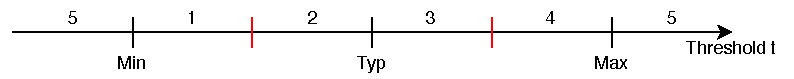
\includegraphics[width=\textwidth]{images/Threshold_Kategorisierung.pdf}
    \caption{Skizziertes Qualitätsmaß anhand der Charakterisierung von Knowm aus Abbildung~\ref{tab:Threshold}.}
    \label{fig:Threshold_Char}
  \end{figure}

\subsection{Qualitätskriterium: Lebensdauer}
  In diesem Abschnitt wird es um die Lebensdauer von Memristoren gehen. Dafür müssen die folgenden zwei Fragen beantwortet werden: Wie kann man die Lebensdauer eines Memristors bestimmen und welchen Einfluss hat die Lebensdauer auf die Qualität des Memristors?

  Wie kann die Lebensdauer eines Memristors also bestimmt werden? Das Team von Knowm betrachtet erst seit der Veröffentlichung der Memristoren der neueren Generation~\cite{knowm_comp_2019} die sogenannte \glqq cycle endurance\grqq. Bei den Memristoren der vorherigen Generationen gab es noch zu wenige Daten dazu.
  \begin{quotation}
    \textit{We currently have limited data on cycling endurance.}
  \end{quotation}
  Sie stellen jedoch fest, dass es einen Zusammenhang zwischen einer höheren Spannung und einer somit kürzeren Lebensdauer geben muss.
  \begin{quotation}
    \textit{Higher voltages will reduce device lifespace.}
  \end{quotation}
  Für die neueren Memristoren gibt es jedoch Abschätzungen für maximale, typische und minimale Lebensdauer~\cite{knowm_comp_2019}, welche im Kapitel~\ref{sec:Chapter4} in diese Arbeit aufgenommen werden.

  Die Arbeit~\cite{stat_lifetime}, auf welche bereits im Kapitel~\ref{sec:Lebensdauer} eingegangen wurde, befasst sich mit der Berechnung der Lebensdauer von Memristoren. Wie in Abbildung~\ref{fig:lebensdauer_chapter3} zu erkennen ist, bezieht sich die Berechnung der Lebensdauer von Memristoren auf den Abstand $\mathcal{K}$ zwischen der HRS (High Resistive State) und LRS (Low Resistive State). Laut den Autoren der Arbeit gilt ein Memristor als nicht mehr funktionsfähig, wenn der Abstand $\mathcal{K}$ einen bestimmten Wert unterschreitet. Dies geschieht zu einem Zeitpunkt $\tau$, welcher wie folgt berechnet werden kann:
  \begin{align}
    \tau = \alpha \times HRS(0) - \beta \times LRS(0)
  \end{align}
  Hierbei stellen $\alpha$ und $\beta$ Koeffizienten dar, welche von einem festgelegten $\mathcal{K}$ für die minimale Differenz zwischen HRS/LRS und dem Abfall beziehungsweise der Steigung von HRS ($slope_{HRS}$) und LRS ($slope_{LRS}$) abhängt. $HRS(0)$ und $LRS(0)$ stehen hierbei für HRS und LRS eines unbenutzten Memristors. Es gilt also den Zeitpunkt $\tau$ zu bestimmen und daraufhin für einen Memristor zu berechnen wie lange es dauert, diesen Zeitpunkt zu erreichen.

  Dafür muss zunächst die Frage geklärt werden in welcher Einheit die Lebensdauer $\tau$ von Memristoren dargestellt wird. Wie in Abbildung~\ref{fig:lebensdauer_chapter3} zu erkennen ist, bezieht sich die Zeitachse auf sogenannte \glqq cycles\grqq. Auch die Arbeit~\cite{nonvolatile}, welche bereits in Kapitel~\ref{sec:Qualität} beschrieben wurde, bezieht sich bei der Lebensdauer von Memristoren auf \glqq write cycles\grqq, übersetzt also \glqq Schreibzyklen\grqq. Dabei nimmt der Autor an, dass die Lebensdauer eines Memristors ungefähr $10^5$ Schreibzyklen umfasst. Somit liegt eine klare Einheit in Form von Schreibzyklen
  vor, sowie eine erste Abschätzung von $\tau$. Eine genauere Bestimmung von $\mathcal{K}$ folgt in Kapitel~\ref{sec:Chapter4}.

  \begin{figure}
    \centering
      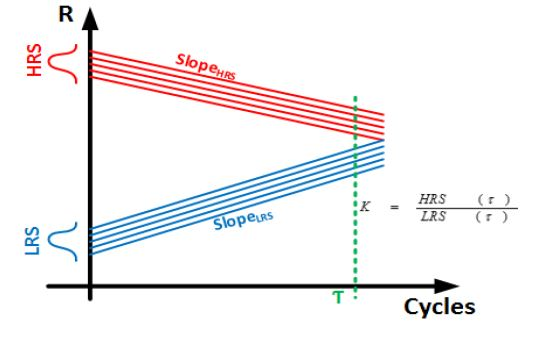
\includegraphics[width=0.7\textwidth]{images/Lebensdauer_Graph.jpg}
      \quelle{\cite{stat_lifetime}}
    \caption{Lebensdauer eines Memristors bis zum Zeitpunkt $\tau$. Der \glqq High Resistive State\grqq\,(HRS) und der \glqq Low Resistive State\grqq\,(LRS) nähern sich während der Lebenszeit eines Memristors an. Bei einem bestimmten Abstand zwischen HRS und LRS gilt der Memristor als nicht mehr funktionsfähig.}
    \label{fig:lebensdauer_chapter3}
  \end{figure}

  Jedoch gibt es mit dieser Lebensdauerabschätzung ein Problem. Die Wissenschaftler, welche diese Daten bereits erhoben haben, nutzen für ihre Arbeit meistens eine Form des Titandioxid-Memristors von HP, während diese Arbeit mit den Memristoren von Knowm arbeitet. Wieso wird diese Möglichkeit der Lebensdauerberechnung also überhaupt vorgestellt? Das liegt daran, dass das Team von Knowm, wie bereits zu Beginn dieses Abschnittes beschrieben, selbst keine näheren Daten als minimale, typische und maximale Gesamtlebensdauer zur Lebensdauer ihrer Memristoren gesammelt hat und somit auf andere Hilfsmittel zugegriffen werden musste. Außerdem betont das Paper~\cite{knowm_comp_2015} einen einzigen wichtigen Unterschied zwischen den Knowm- und den HP-Memristoren: Die Eigenschaft, dass sich Knowm Memristoren nicht so einfach von ihrer Umgebung beeinflussen lassen wie die auf Oxidation basierenden HP-Memristoren. Die Knowm Memristoren sollen sehr ähnlich in der Funktionsweise und in der Eigenschaft im Vergleich zu den HP-Memristoren sein, dabei aber den großen Vorteil haben, dass sie für Forschungszwecke massentauglicher sind, da man nicht in einer sterilen und anderweitig aufwendigen Forschungsumgebung arbeiten muss. HP-Memristoren haben laut den Knowm Entwicklern den Ruf, dass sie sich sehr leicht von äußeren Umständen manipulieren lassen und somit nicht geeignet sind, um in studentischer oder ähnlicher Forschungsarbeit genutzt zu werden. Da es unmöglich ist die Lebensdauer eines Memristors auf den Schreibzyklus genau zu bestimmen und es sich dabei immer um eine Approximation  handelt, scheint es sinnvoll eine bereits im Rahmen einer wissenschaftlichen Arbeit festgestellte Berechnungsvorschrift eines etwas anderen Gerätes zu nutzen und auf diese Bedingungen anzupassen, als einen willkürlichen eigenen Ansatz zu wählen.

  Ein andere Möglichkeit wäre es, einen der zur Verfügung gestellten Memristoren von Knowm zur Aufstellung einer Statistik für die Lebensdauer zu nutzen. Dafür müsste für den ausgewählten Memristor davon ausgegangen werden, dass er nahezu unbenutzt ist. Damit könnte eine Messreihe gestartet werden, die wie folgt auszusehen hat: Für den Memristor muss immer nach einem Schreibzyklus der HRS und LRS, also der maximale und minimale Widerstand, ausgemessen und in einer Statistik festgehalten werden. Es sollte dabei ein ähnlicher Graph, wie in Abbildung~\ref{fig:lebensdauer_chapter3} entstehen. Sobald die Daten erhoben wurden, sollte der genutzte Memristor nicht mehr funktionsfähig sein. Der Zeitpunkt, zu dem die Funktionsfähigkeit aufgehört hat, muss daraufhin bestimmt werden. Damit liegt dann der Zeitpunkt $\tau$ mit dem Abstand $\mathcal{K}$ zwischen HRS und LRS vor.

  Bei beiden Möglichkeiten liegt ein Graph wie in Abbildung~\ref{fig:lebensdauer_chapter3} vor, welcher nun genutzt werden kann, um die restliche Lebensdauer jedes weiteren Memristors zu approximieren. Dafür könnte eine Funktion aufgestellt werden, welche den Abstand zwischen HRS und LRS bis zum Zeitpunkt $\tau$ darstellt. Zum Bestimmen der Lebensdauer kann für jeden Memristor durch das Ausmessen des maximalen und minimalen Widerstands der daraus resultierende Abstand zwischen beiden bestimmt werden. Der Abstand kann nun zusammen mit der zuvor aufgestellten Funktion genutzt werden, um die restliche Lebensdauer des betrachteten Memristors zu bestimmen.

  Nun soll es um den Einfluss der restlichen Lebensdauer auf die Qualität des Memristors gehen. Die Restlebensdauer wird in dem Qualitätsmaß, welches im Zuge dieser Arbeit erstellt wird, eine spezielle Rolle spielen. Einerseits sollte die Lebensdauer keine Rolle für die Qualität des Memristors spielen, wenn der Memristor noch für viele Schreibzyklen funktionsfähig sein wird. Ein Memristor von minderer Qualität sollte in diesem Qualitätsmaß nicht eine höhere Qualität erhalten, weil er eine längere Restlebensdauer hat, als ein qualitativ hochwertigerer Memristor mit weniger Restlebensdauer. Andererseits jedoch, sollte eine sehr kurze restliche Lebensdauer einen relativ hohen Einfluss auf die Gesamtqualität des Memristors haben. Ein hochqualitativer Memristor, welcher nicht mehr viele Schreibzyklen funktionieren wird, sollte diese Tatsache zur Ermittlung der Qualität in Betracht ziehen. Es bietet sich also an, einen Zeitpunkt zu finden, an welchem ein Memristor nach der bestimmten Anzahl von Schreibzyklen an Qualität verliert. Genauere Werte dazu folgen in Kapitel~\ref{sec:Chapter4}.

  Eine Frage kommt jedoch mit der Betrachtung der Lebensdauer in Hinblick auf die Qualität hinzu. Gibt es einen direkten Zusammenhang zwischen Lebensdauer und Qualität? In der Arbeit~\cite{stat_lifetime} wurde klar definiert, dass die Lebensdauer vom Abstand zwischen dem HRS und LRS abhängt. Jedoch liegt es nahe, dass auch die Qualität des Memristors mit der Zeit abnimmt, wenn sich \glqq High Resistive State\grqq\,und \glqq Low Resistive State\grqq\,immer weiter annähern und damit möglicherweise die Anzahl der Zustände schrumpft. Zum aktuellen Zeitpunkt liegen dazu keinerlei Daten vor. Doch sie werden in Kapitel~\ref{sec:Chapter5} der Evaluation noch einmal aufgegriffen.

\subsection{Qualitätskriterium: Formbarkeit}
  In diesem Abschnitt soll auf die sogenannte \glqq Formbarkeit\grqq\,von Memristoren eingegangen und der Einfluss auf die Qualität analysiert werden. Was man unter der Formbarkeit von Memristoren versteht, wurde bereits in Kapitel~\ref{sec:Formbarkeit} beschrieben, doch wie kann man sie kategorisieren? Dafür muss zunächst untersucht werden, was es bedeutet, dass ein Memristor eine gute Formbarkeit besitzt. Da Formbarkeit immer in Relation zu einem zweiten Memristor oder einer bestimmten Hysterese steht, ist es nicht so einfach eine allgemeine Formbarkeit zu kategorisieren.

  Bei der Formbarkeit geht es darum, dass ein Memristor die Voraussetzung besitzt, in die gleiche \glqq Form\grqq\,eines anderen Memristor \glqq geformt\grqq\,zu werden. Um das jedoch allgemein kategorisieren zu können, kann schlecht eine bestimmte Form angenommen werden, da diese nicht unbedingt bedeutet, dass sich dieser Memristor dazu eignet, in die vom Nutzer gewünschte Form gebracht zu werden. Wie bringt man die Formbarkeit eines Memristors also am besten in dieses Qualitätsmaß ein? Es muss beim Kategorisieren auf eine allgemeine Formbarkeit geachtet werden, also ob es möglich ist, diesen Memristor in möglichst viele verschiedene Formen zu bringen.

  In dem Abschnitt~\ref{sec:Vergleich} geht es um den Vergleich von den Hysteresen zweier Memristoren. Dieser Vergleich kann für diesen Aufgabenbereich mit kleinen Veränderungen verwendet werden. Einerseits wird nicht der Vergleich von zwei Hysteresen von unterschiedlichen Memristoren vollzogen, sondern ein Vergleich von zwei Hysteresen des gleichen Memristors, wobei unterschiedliche Amplituden angelegt werden. Auch wird für das Qualitätsmaß nicht nach einer möglichst nahen Ähnlichkeit gesucht, sondern nach einem möglichst hohem Unterschied in den Hysteresen. Je unterschiedlicher die Hysteresen des jeweilig betrachteten Memristors sind, umso formbarer ist er auch. Konkrete Werte, ab welchen ein Memristor nach der Abstandsfunktion als \glqq formbar\grqq\,gibt, gibt es im Kapitel~\ref{sec:Chapter4}.


  Eine weitere wichtige Rolle in der Formbarkeit eines Memristors spielt unter anderem das sogenannte \glqq Conditioning\grqq. Bei diesem Vorgang kann man auch vom \glqq Wiederbeleben\grqq\,eines Memristors sprechen. Beim Conditioning wird mit einer relativ hohen Spannung ein Puls auf einen Memristor geschickt, welcher einen sehr dünnen Hysteresen-Loop hat. Durch den Puls kann es passieren, dass der Loop der Hysterese aufgeweitet wird und der Memristor somit wieder funktionsfähig wird. Abbildung~\ref{fig:Hysteresen} zeigt hierbei in a) und b) wie das Aufweiten einer Hysterese in der Praxis in etwa auszusehen hat. Dabei gibt es natürlich einen direkten Zusammenhang zwischen Qualität und Conditioning. Während ein Memristor mit einem nahezu nicht vorhandenem Loop in der Hysterese vermutlich qualitativ als nicht funktionsfähig eingestuft werden kann, da eine \glqq Gerade\grqq\,als Hysterese impliziert, dass der Memristor bei Anlegen der Spannung keinen nennenswerten Zustandsübergang hat, liegt nach einem erfolgreichem Conditioning ein wieder funktionsfähiger Memristor vor.

  Es liegt also nahe, einen Memristor zu Beginn des Qualitätschecks darauf zu überprüfen, ob er einen geweiteten Hysteresen-Loop besitzt. Ist dieser bereits aufgeweitet, so kann einfach der normale Qualitätscheck starten und die Formbarkeit kann in diesem Zuge auch normal wie beschrieben kategorisiert werden. Ähnelt die Hysterese zu Beginn eher einer Geraden oder ist allgemein sehr wenig geweitet, sollte zunächst versucht werden, den Memristor durch Conditioning \glqq wiederzubeleben\grqq. Gelingt dies nicht braucht es keine weiteren Tests, um festzustellen, dass der Memristor von niedriger Qualität ist. Gelingt das Conditioning, kann daraufhin der normale Qualitätscheck fortgeführt werden.

  \begin{figure}
    \centering
    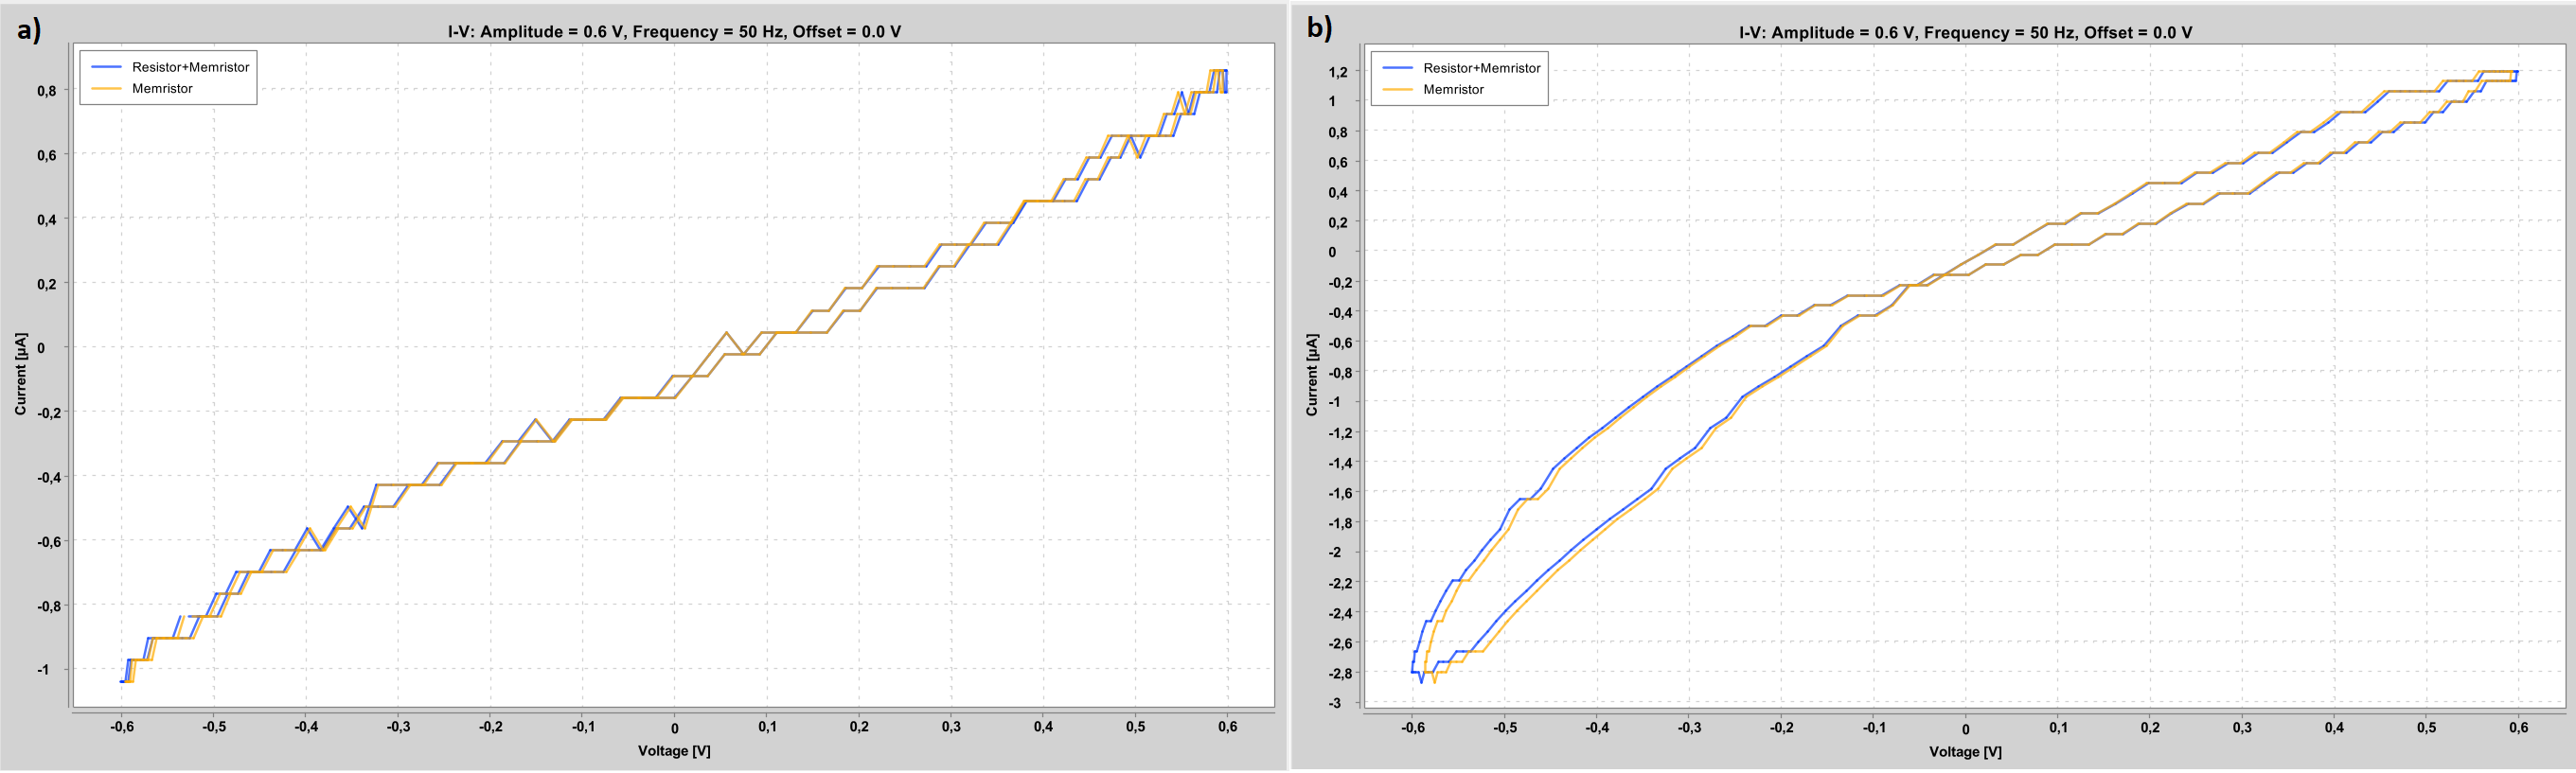
\includegraphics[width=\textwidth]{images/Conditioning.png}
    \caption{Conditioning: a) Hysterese eines nicht funktionsfähigen Memristors b) Hysterese des gleichen Memristors nach einem durchgeführten Conditioning.}
    \label{fig:Hysteresen}
  \end{figure}

\subsection{Aufstellung des Qualitätsmaßes}
In diesem Abschnitt werden alle vorangegangen Abschnitte genutzt, um ein konkretes Qualitätsmaß zu erstellen. Alle Qualitätskriterien erhalten hierbei die gleiche Priorität. Zwar kann argumentiert werden, dass für ein allgemeines Qualitätsmaß die Speichergröße von höherer Relevanz ist, als zum Beispiel die Formbarkeit. Diese bezieht sich mehr auf den Vergleich von zwei Memristoren und nicht auf die Qualität eines bestimmten Memristors. Jedoch wird in der fertigen Implementierung eine Ausgabe jeder Teilnote zur Verfügung gestellt. Dementsprechend gibt es keine unterschiedliche Priorität zwischen den Qualitätskriterien. Jeder Nutzer kann sich eine eigene Priorität jedoch selbst aus den gegebenen Teilnoten herleiten.

Für die Approximation der Restlebensdauer als Qualitätskriterium gilt immer dasselbe. Die Lebensdauer hat die Eigenschaft, dass sie entweder gar keinen oder einen relativ großen Einfluss auf die Qualität hat. Ist die Restlebensdauer eines Memristors noch sehr hoch, so ist für seine Qualität nur davon abhängig, wie gut die anderen Faktoren benotet sind. Ist die Restlebensdauer eines Memristors sehr niedrig, so können alle anderen Faktoren gut benotet sein, der Memristor wird nach einiger Zeit trotzdem funktionsunfähig werden. Um diese Qualitätskriterien in das Qualitätsmaß einzubeziehen, muss der Ablauf zur Generierung der Gesamtnote betrachtet werden.

\begin{figure}
  \centering
  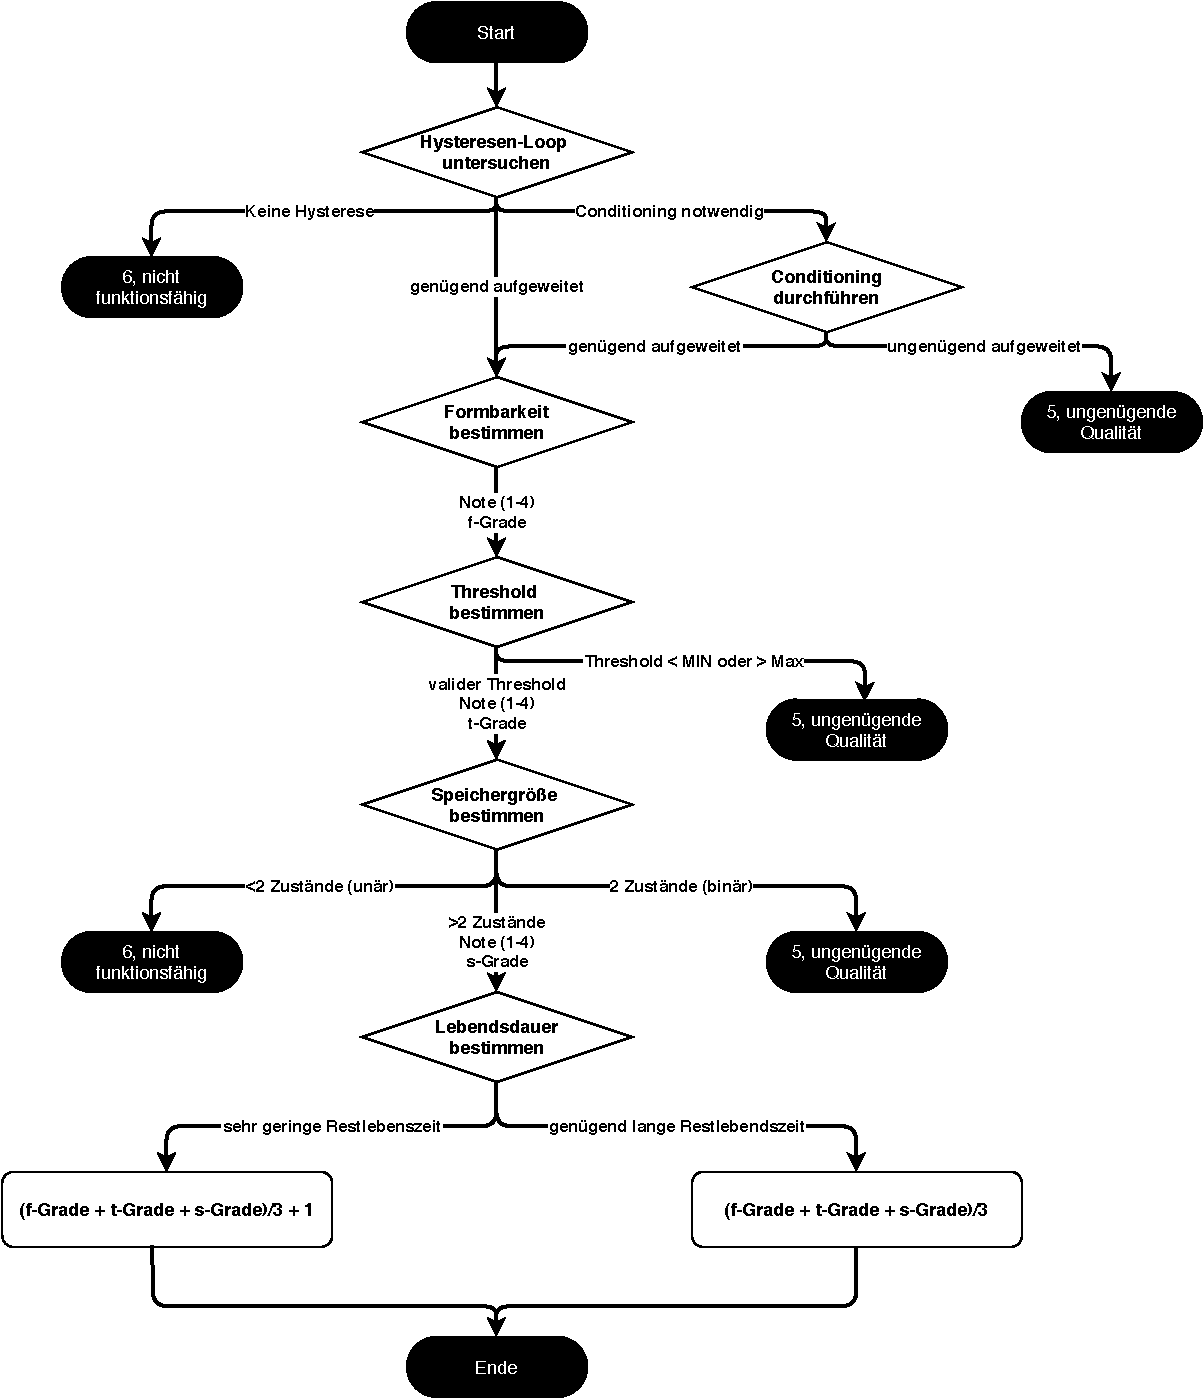
\includegraphics[width=\textwidth]{images/Notengeneration.pdf}
  \caption{Der Ablauf zur Aufstellung des Qualitätsmaßes mit der Generierung der Noten eines Memristors.}
  \label{fig:Notengenerierung}
\end{figure}

Der Ablauf ist in Abbildung~\ref{fig:Notengenerierung} dargestellt. Zuallererst wird die Formbarkeit eines Memristors untersucht. Besitzt der Memristor keine Hysterese, so braucht auch keine Formbarkeit oder Qualität getestet werden. Der Memristor ist nicht funktionsfähig und wird mit der Note 6 bewertet. Ist eine Hysterese vorhanden, der Loop jedoch nicht geweitet genug, so gibt es zwei Möglichkeiten. Lässt sich der Memristor auch mit Conditioning nicht wieder aufweiten, so kann der Prozess zur Qualitätsbestimmung direkt abgebrochen und der Memristor mit ungenügender Qualität und der Note 5 deklariert werden. Ist es möglich ihn mit Conditioning aufzuweiten, so kann, genau wie im Falle, dass die Hysterese zu Beginn bereits genug aufgeweitet ist, die Qualitätsbestimmung fortgesetzt werden.

Nun können Threshold und Speicherkapazität bestimmt und benotet werden. Bei der Bestimmung dieser beiden Qualitätskriterien muss der maximale und minimale Widerstand des Memristors bestimmt werden, woraus sich die Restlebensdauer ableiten lässt. Der Einfluss der Lebensdauer auf die Qualität ist wie bereits beschrieben nur vorhanden, wenn die restliche Lebenszeit des Memristors gering ist. Im Ablauf der Notengeneration teilt sich das Ergebnis hier also einmal in zwei Fälle auf.

Insgesamt lässt sich nach Ablauf zur Bestimmung der Gesamtnote des Memristors mit der folgenden Formel berechnen.
\begin{align*}
  \label{align:Quality}
  \text{Qualität } = \frac{\text{s-Grade} + \cdot \text{t-Grade} + \text{f-Grade}}{3} + L
\end{align*}
Hierbei stellt \glqq s-Grade\grqq\,die Note für das Qualitätsmaß der Speicherkapazität dar. Der Energieverbrauch, welcher anhand des Thresholds bestimmt wird, wird anhand der \glqq t-Grade\grqq\,benotet. Das Qualitätsmaß für die Formbarkeit erhält die Note \glqq f-Grade\grqq. Die Variable $L$ hängt von dem Qualitätskriterium der Lebensdauer ab. Dabei soll als Zeitpunkt, ab welchem der Memristor eine für das Qualitätsmaß zu niedrige Restlebensdauer besitzt, $10\%$ der Gesamtlebensdauer gewählt werden. Die Gesamtlebensdauer lässt sich wie folgt darstellen:
\begin{align*}
  L = \begin{cases}
    1, &\text{ wenn die Restlebensdauer kürzer ist als 10\% der Gesamtlebensdauer}\\
    0, &\text{ sonst}
  \end{cases}
\end{align*}
 Wie in der Abbildung~\ref{fig:Notengenerierung} zu erkennen ist, liegen s-Grade, t-Grade und f-Grade immer zwischen 1 und 4. Dadurch bildet sich mit der Formel~\ref{align:Quality} eine Note zwischen 1 und 5. Die Note 6 kann nur durch einen vorzeitigen Abbruch des Ablaufs entstehen. Ein Memristor kann nicht durch den gesamten Ablauf der Notengenerierung kommen und danach mit der Note 6 als nicht funktionsfähig beschrieben werden. Da der Memristor durch den Prozess der Notengenerierung gekommen ist, kann davon ausgegangen werden, dass er funktionsfähig ist, auch wenn die Qualität sehr schlecht ist. Deshalb ist die schlechteste Note in diesem Fall 5.

\section{Ähnlichkeiten zwischen Memristoren}
\label{sec:Vergleich}
In diesem Abschnitt wird auf den Vergleich von zwei Memristoren eingegangen. Beim Vergleich von Memristoren gibt es einige Aspekte die betrachtet werden müssen. Dafür muss untersucht werden, was es bedeutet, dass zwei Memristoren \glqq gleich\grqq\,sind. Anhand welcher Merkmale kann ein Memristor mit einem anderen Memristor verglichen werden? Hierfür können die im vorherigen Teilkapitel angesprochenen Qualitätskriterien eingebunden werden.

Die Lebensdauer hat in der Betrachtung von Ähnlichkeiten zweier Memristoren eine untergeordnete Rolle. Zwar kann es Anwendungsgebiete geben, in denen es wichtig ist, dass die Memristoren eine ähnlich lange Lebensdauer haben, jedoch sollte diese Betrachtung unabhängig zu der eigentlichen Analyse von Gemeinsamkeiten ablaufen. Sind zwei Memristoren sehr ähnlich zueinander, ihre restliche Lebensdauer jedoch sehr unterschiedlich, müssen die beiden Memristoren trotzdem als \glqq ähnlich\grqq\,klassifiziert werden. Eine gleiche Lebensdauer sollte dabei als nebensächlich gelten.

Ein wichtigerer Faktor für Ähnlichkeiten zwischen zwei Memristoren ist die Anzahl von Zuständen. Eine gleiche Anzahl an Zuständen ist in vielen Anwendungsgebieten von Memristoren ein wichtiger Faktor. Einerseits muss bei dem Vergleich darauf geachtet werden, wie groß der Abstand der Zustandsanzahl von beiden Memristoren ist. Hat ein Memristor zum Beispiel vier Zustände und der zu vergleichende Memristor acht Zustände, ist der Abstand hier vier. Andererseits muss jedoch auch in Betracht gezogen werden, ob die Memristoren sich um eine Zweierpotenz unterscheiden. In dem gerade genannten Beispiel wäre dies der Fall, da der Memristor mit vier Zuständen zwei Bit kodieren kann, also in die Klasse von $2^2$ gehört, ein Memristor mit acht Zuständen drei Bit kodieren kann, somit zu einer anderen Zweierpotenz, hier $2^3$, gehört. Bei der Betrachtung von Ähnlichkeiten zwischen zwei Memristoren in Hinblick auf die Anzahl an erreichbaren Zuständen, muss also auf zwei Faktoren geachtet werden: Der direkte Abstand in Form von der Anzahl an Zuständen und der Abstand zwischen den \glqq Zweierpotenzklassen\grqq.

Der nächste Faktor zur Ähnlichkeit, welcher betrachtet werden muss, ist der Threshold. Für einige Anwendungen kann es wichtig oder zumindest von Vorteil sein, dass beide Memristoren mit einer gleich hohen Spannung gesetzt werden können. Hierbei muss zunächst von beiden Memristoren der Threshold $t_1$ und $t_2$ ermittelt werden. Danach kann mit der einfachen Rechnung $| t_1 - t_2 |$ der Abstand zwischen den beiden Thresholds bestimmt und somit die Ähnlichkeit der Memristoren mit einem weiteren Faktor kategorisiert werden.

Der jedoch wichtigste Faktor für die Ähnlichkeit von zwei Memristoren ist die Formbarkeit. Hierbei wird aber nicht wie im vorherigen Teilkapitel eine allgmeine Formbarkeit untersucht, sondern eine konkrete Formbarkeit in Bezug auf einen spezifischen Memristor. Es ist in dieser Betrachtung also unwichtig, wie hoch die Qualität des Memristors in Bezug auf die Formbarkeit ist. Es wird hierbei viel mehr eine Form überprüft und festgestellt, ob diese von dem betrachteten Memristor erreichbar ist. Dabei werden zwei Hysteresen, die Hysterese des betrachteten Memristors, welche verändert werden kann und die Hysterese des zu erreichenden Memristors, welche starr bleibt, wie in Abbildung~\ref{fig:Hysteresenvergleich} untersucht. Als Maß für die Ähnlichkeit der beiden Hysteresen wird eine Abstandsfunktion definiert.

Zum Aufstellen der Abstandfunktion muss die Hysterese als Graph in einem Koordinatensystem betrachtet werden. Die Achsen bleiben hierbei die Stromstärke und die Spannung. Dabei wird der Graph, wie in Abbildung~\ref{fig:Hysteresenfunktionen}, an den Wendepunkten des Graphen in zwei Funktionen aufgeteilt. Macht man dies bei beiden zu vergleichenden Hysteresen, erhält man vier Funktionen $f_1, f_2, f_3, f_4$. Sind diese Funktionen aufgestellt, muss nun nur noch der Abstand zwischen den Werten der Funktionen $f_1$ und $f_3$, sowie $f_2$ und $f_4$ aufgestellt werden. Der Abstand $\mathcal{A}$ der beiden Hysteresen lässt sich also annähernd wie folgt Bestimmen:

\begin{align}
  \mathcal{A} = \sum_{x = - \infty}^\infty (f_1(x) - f_3(x)) + \sum_{x = - \infty}^\infty (f_2(x) - f_4(x))
\end{align}

Diese Formel ist rein konzeptuell und wird in der Implementierung zwar nach einem sehr ähnlichen Prinzip berechnet, jedoch muss dabei noch auf unterschiedliche Faktoren geachtet werden. Zum Beispiel lässt sich dabei die Summe statt für $x=-\infty$ bis $\infty$ mit eine einfacheren Abschätzung darstellen, da die Spannungswerte bestimmte Schranken nicht überschreiten. Auch sollten keine ganzzahligen Abstände zwischen den $x$ der Summe gewählt werden, da somit die Genauigkeit des Abstands verloren gehen könnte. Zur Implementierung des Vergleichs und der Abstandsfunktion im Detail wird mehr im Kapitel~\ref{sec:Chapter4} beschrieben.

\begin{figure}
  \centering
  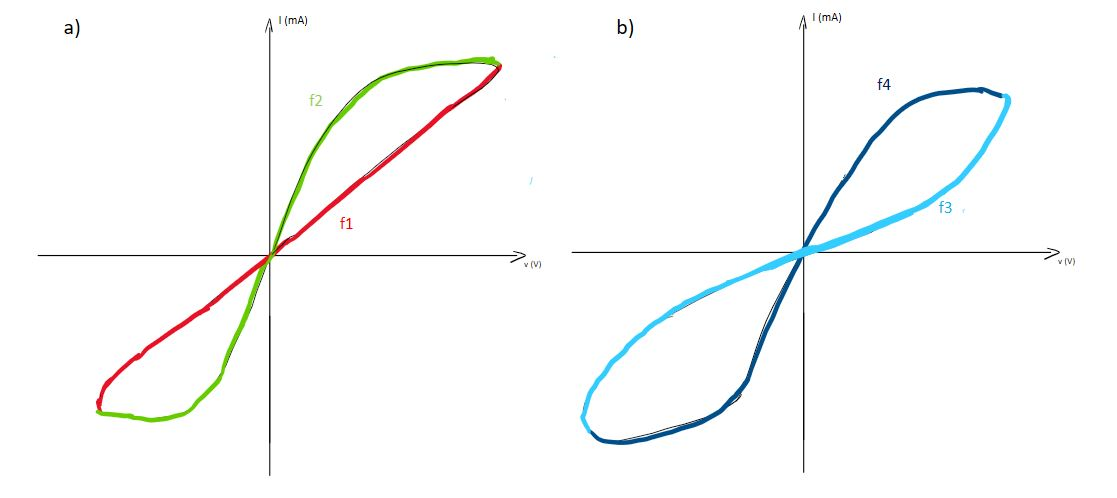
\includegraphics[width=0.9\textwidth]{images/Hysteresenfunktionen}
  \caption{Skizze zum Aufteilen der Hysteresen in vier Funktionen, welche daraufhin einfach verglichen werden können. a) die erste Hysterese mit Funktionen $f_1$ und $f_2$ b) die zweite Hysterese mit Funktionen $f_3$ und $f_4$.}
  \label{fig:Hysteresenfunktionen}
\end{figure}

Anhand dieser Abstandsfunktion kann nun entschieden werden, ob die Hysteresen eine Ähnlichkeit besitzen. Dafür muss ein spezifischer Schwellenwert definiert werden, ab welchem zwei Memristoren als ähnlich gelten. Sollten sich die beiden Hysteresen nicht genügend ähneln, so muss durch das Anlegen einer anderen Amplitude oder eines anderen Offsets auf den betrachteten Memristor die Hysterese verändert werden und der Vergleich wiederholt werden. Gibt es eine bestimmte Form des betrachteten Memristors, für welche die beiden Memristoren als ähnlich gelten, so kann die Untersuchung mit einem positiven Ergebnis abgebrochen werden. Die Memristoren besitzen also eine genügende Ähnlichkeit. Ist es für alle untersuchten Hysteresen des betrachteten Memristors nicht möglich, eine Ähnlichkeit zu finden, so bedeutet das jedoch nicht sofort, dass keine Ähnlichkeit zwischen den beiden Memristoren herrscht. Sie gleichen sich zwar nicht anhand ihrer Hysteresen, wodurch sie für einige Einsatzgebiete nicht zusammen genutzt werden sollten, jedoch gibt es wie bereits beschrieben auch andere Faktoren für die Ähnlichkeit von zwei Memristoren. Somit kann nach einem negativen Ergebnis im Vergleich der Hysteresen immer noch untersucht werden, wie sehr sich die Anzahl an Zuständen und der Threshold zum Setzen des Memristors zueinander verhält. Beide Faktoren können hierbei wie bei der Qualitätsbestimmung definiert werden und dann direkt verglichen werden. Hierbei muss zwar festgehalten werden, dass sie sich in Bezug auf ihre Hysteresen nicht ähneln, sie jedoch an einer anderen Stelle vielleicht eine gewisse Ähnlichkeit besitzen, was für bestimmte Anwendungsgebiete ausreichend sein kann.

\begin{figure}
  \centering
  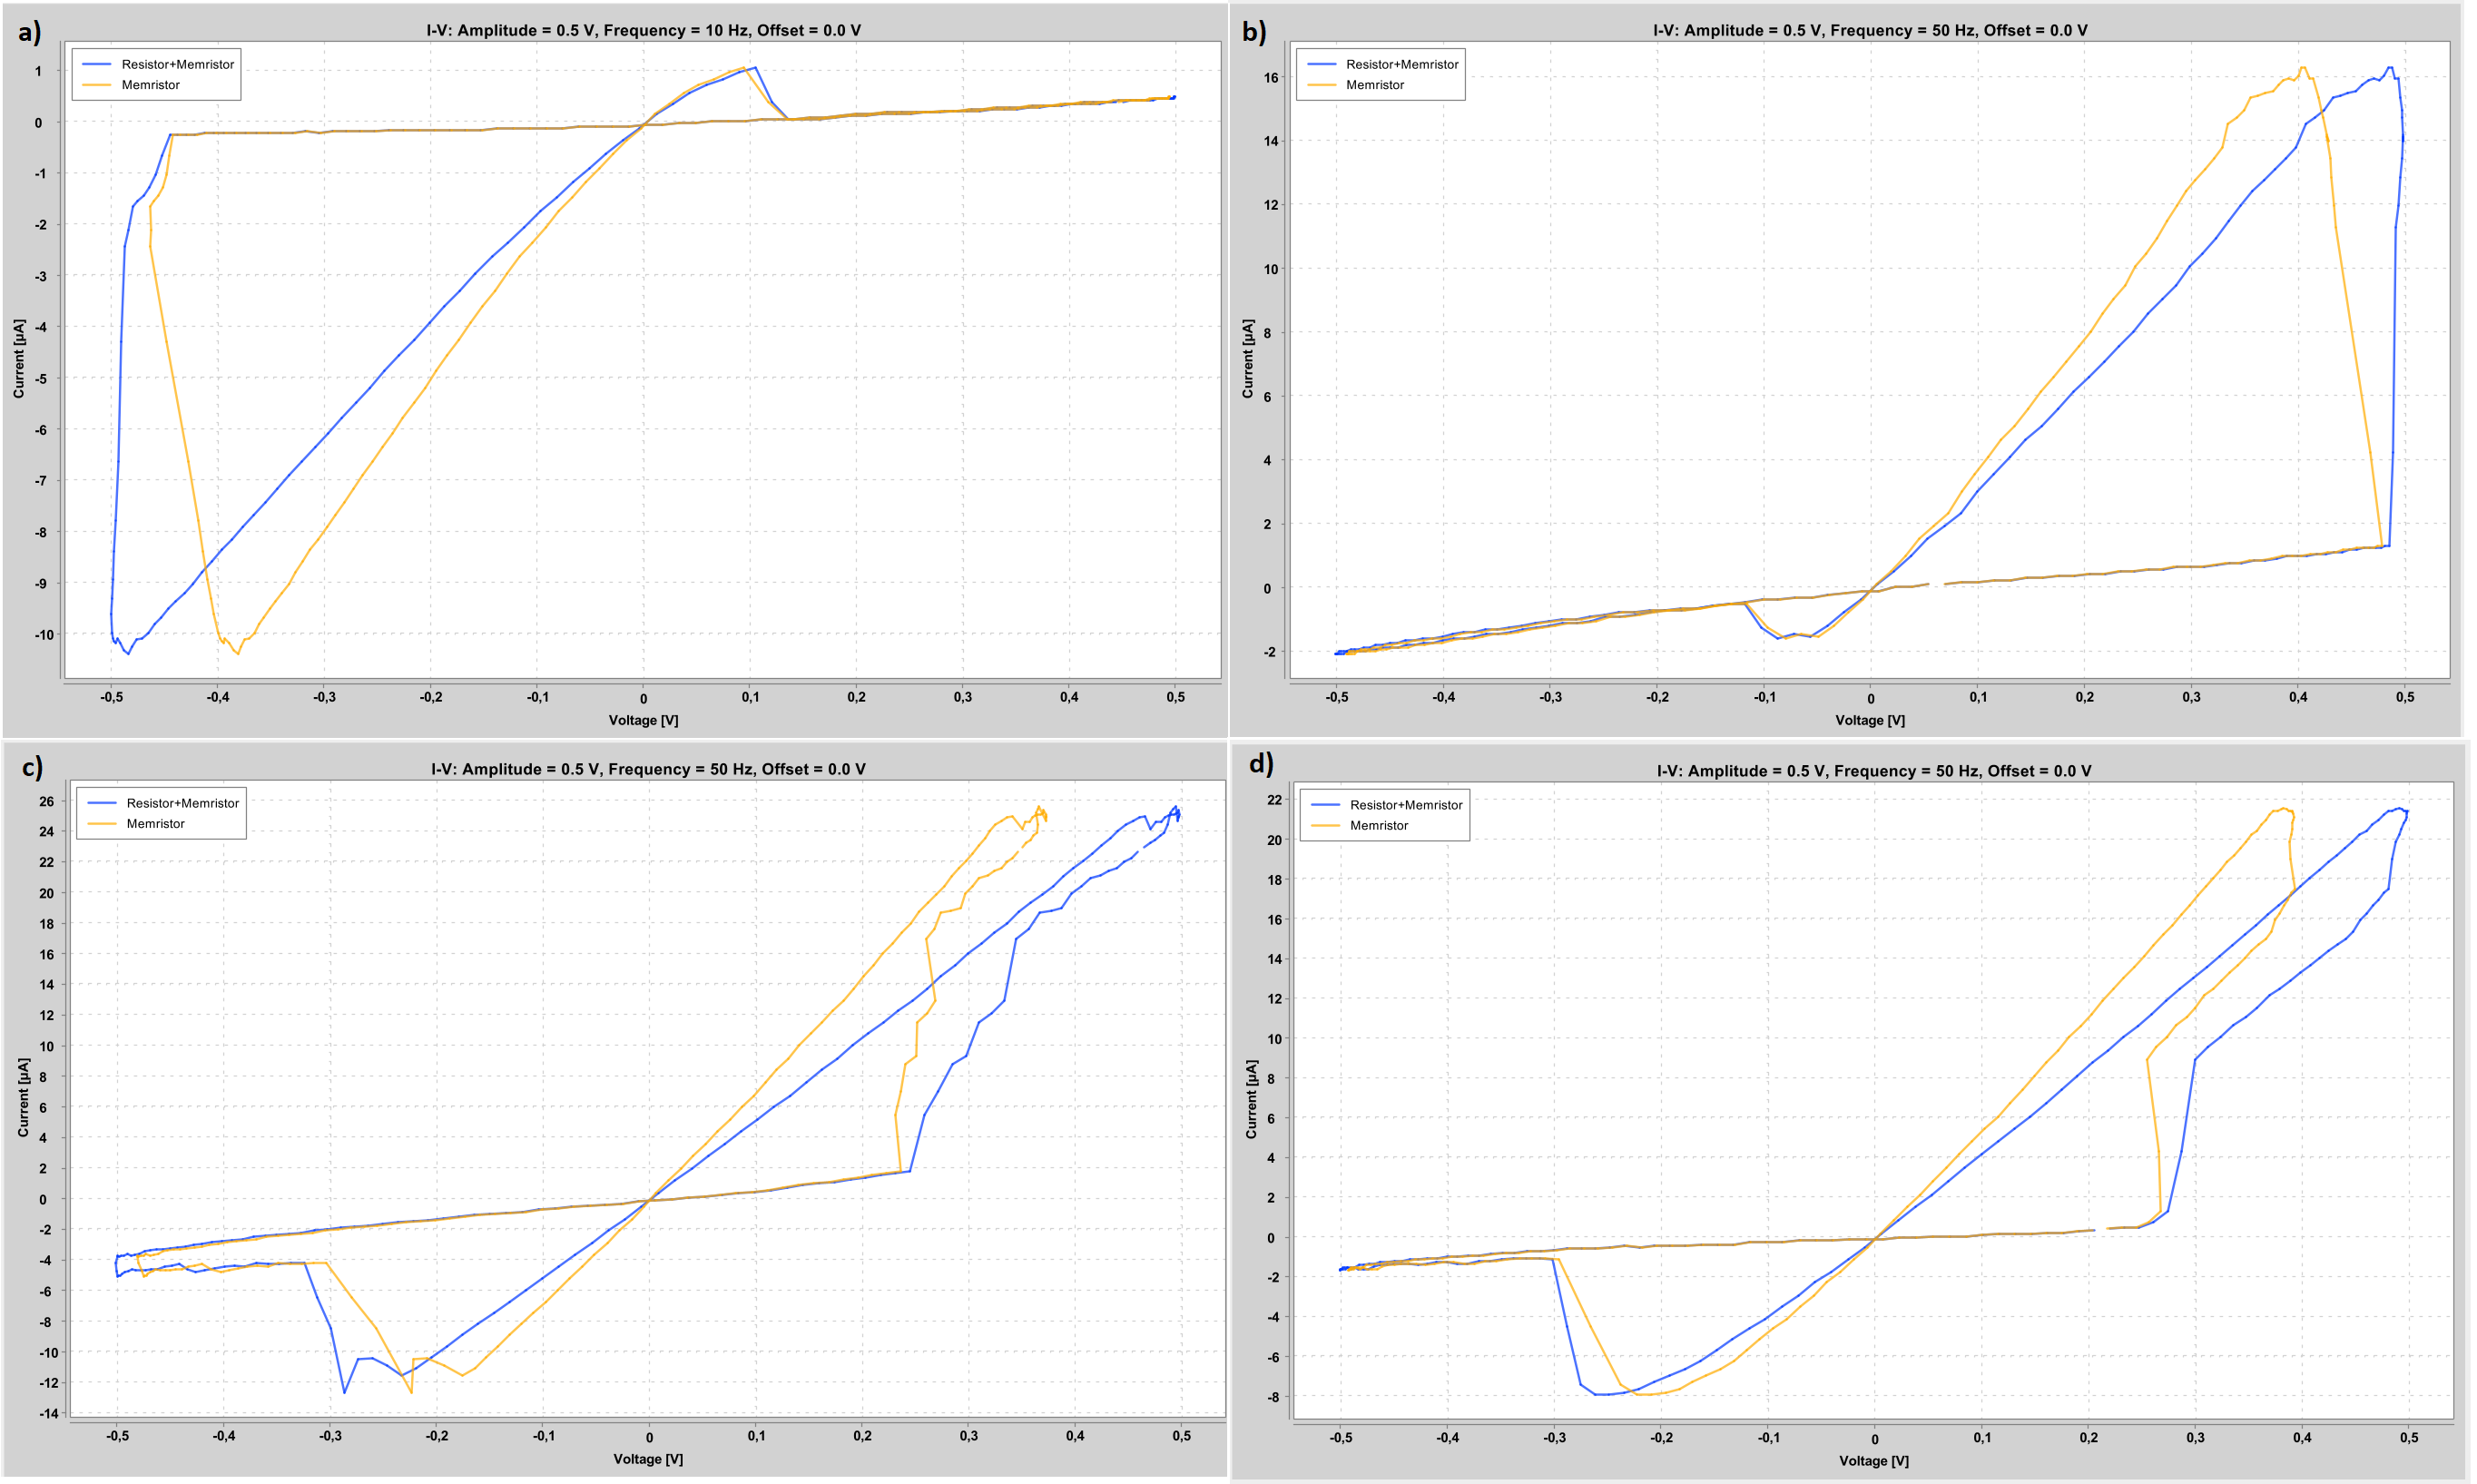
\includegraphics[width=0.95\textwidth]{images/Hysteresen_Vergleich}
  \caption{Beispielhysteresen für Vergleich: Die Hysteresen aus a) und b) unterscheiden sich sehr stark, die Hysteresen aus c) und d) besitzen dagegen eine gewisse Ähnlichkeit.}
  \label{fig:Hysteresenvergleich}
\end{figure}
Wenn die drei relevanten Faktoren für die Ähnlichkeit von zwei Memristoren zusammengeführt werden, kann eine Kategorisierung wie folgt aussehen. Da der Faktor der Formbarkeit die anderen beiden Faktoren in Relevanz klar übersteigt, muss zuallererst auf die Formbarkeit geachtet werden. Wenn es möglich ist, den betrachteten Memristor in den anderen zu \glqq formen\grqq\,und somit zwei sehr ähnliche Hysteresen vorliegen, verlieren die beiden anderen Faktoren stark an Relevanz. Ist es nicht möglich, gleiche Hysteresen zu formen, so kann zumindest ein Vergleich von Speichergröße und Energieverbrauch aufgestellt werden. In dem Fall kann es zwar sein, dass sich die beiden Memristoren nicht direkt anhand ihrer Hysterese ähneln, jedoch könnte einer der beiden gerade genannten Faktoren ähnlich sein und somit eine etwas schwächere Ähnlichkeit existieren.

\begin{figure}
  \centering
  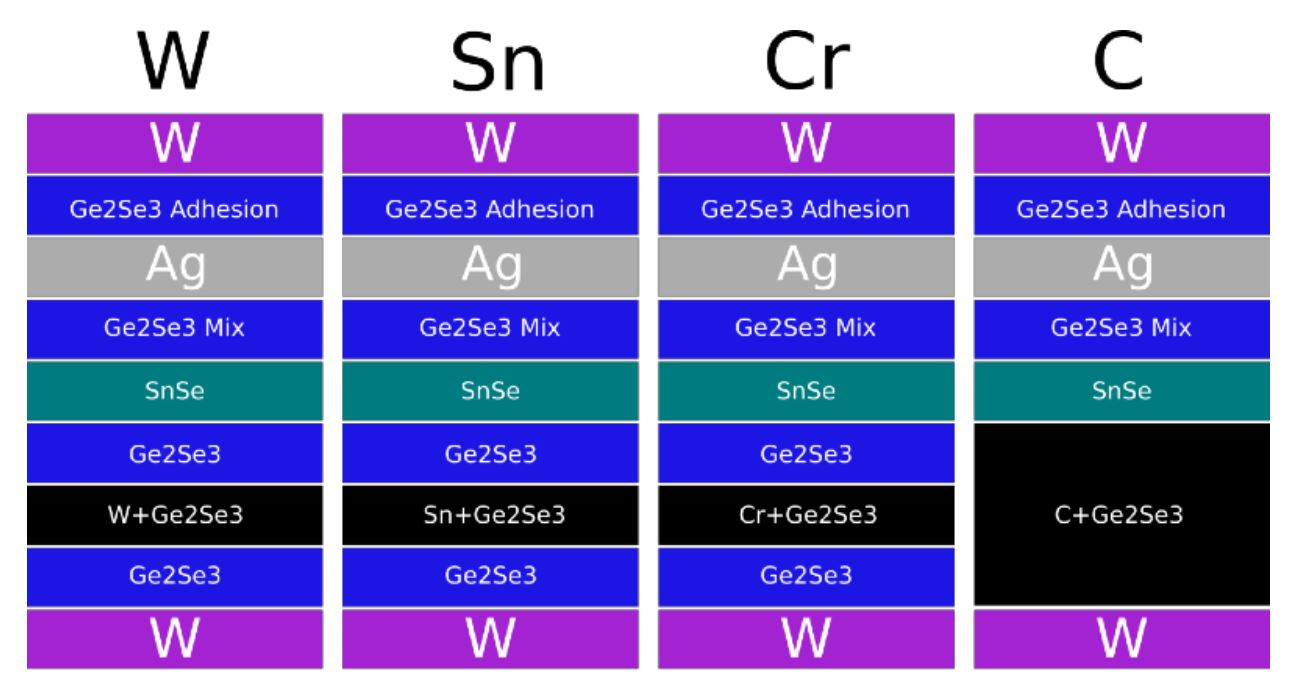
\includegraphics[width=0.85\textwidth]{images/Materialien.jpg}
  \quelle{\cite{knowm_comp_2019}}
  \caption{Verschiedene Materialen (Wolfram, Zinn, Chrom, Kohlenstoff) des Memristors von Knowm Inc.}
  \label{fig:mem_materialien}
\end{figure}

\section{Einfluss des Materials auf die Qualität}

In diesem Abschnitt wird auf unterschiedliche Materialien für Memristoren eingegangen. Knowm Inc. stellt ihre Memristoren im Grunde in drei verschiedenen Ausführungen für den Verkauf zur Verfügung. Dabei unterscheiden sich diese nur in der Wahl der Materialien, aus welchen der Memristor besteht. Es gibt hierbei Wolfram, Chrom und Zinn als verschiedene Materialien. Es gibt auch noch eine vierte Art Memristor, welche auf Kohlenstoff basiert, jedoch fehlen diesem Modell einige wichtige Eigenschaften, wie zum Beispiel das Speichern von mehreren Bits in einem Baustein, weshalb er in dieser Arbeit nicht zum Vergleich herangezogen wird. Im Datenblatt von Knowm (Datasheet in~\cite{knowm_comp_2019})
gibt es bereits einige Angaben zu den unterschiedlichen Materialen. Zum Beispiel variieren maximaler und minimaler Threshold zwischen dem Chrom Memristor und den anderen Arten. Auch haben die Memristoren unterschiedliche HRS/LRS. Der Einfluss der verschiedenen Materialien auf die Qualität des Memristors kann jedoch nur mit eigenen Messungen überprüft werden. Genauere Angaben hierzu sind im Kapitel~\ref{sec:Chapter5} in den Ergebnissen zu finden.
